%%% Local Variables:
%%% coding: utf-8
%%% mode: latex
%%% TeX-engine: xetex
%%% End:
\documentclass[10pt,notes]{beamer}
% NOTE May need to manually set tex engine in emacs

\usetheme[progressbar=frametitle]{metropolis}
\usepackage{appendixnumberbeamer}
\usepackage{svg}
\usepackage{ulem}
\usepackage{scalerel}
\usepackage{cancel}
\usepackage{wrapfig}
\usepackage{fancyvrb}
\usepackage{hyperref}
\hypersetup{
    colorlinks = true,
    linkcolor = blue
    }
\usepackage{cleveref}
\usepackage{stmaryrd}
\usepackage{amsmath}
\usepackage{amssymb}
\usepackage{listings}
\usepackage{pdfpc}
\usepackage{textcomp}
\newcommand<>{\talknote}[1]{\only#2{\pdfpcnote{- #1}\relax}}

\usepackage{pifont}
\newcommand{\cmark}{\ding{51}}
\newcommand{\xmark}{\ding{55}}

\usepackage[dvipsnames]{xcolor}
\definecolor{mLightGreen}{HTML}{14B03D}

\usepackage{booktabs}
\usepackage[scale=2]{ccicons}

\usepackage{graphicx}

\usepackage{pgfplots}
\usepgfplotslibrary{dateplot}

\usepackage{todonotes}
\newif\ifdraft
\drafttrue
\newcommand{\todoin}[1]{\ifdraft{\todo[inline]{TODO:\@ #1}}\fi}

\usepackage{xspace}
\usepackage{mathpartir}
\newcommand{\themename}{\textbf{\textsc{metropolis}}\xspace}

\newsavebox{\logoagdabox}
\sbox{\logoagdabox}{%
  %
  \raisebox{-2pt}{
\includegraphics[height=1em]{logo-agda.pdf}}%
}
\newcommand{\agdalogo}{%
  \usebox{\logoagdabox}}%


\newcommand{\Agda}{\agdalogo}
\usepackage[LGR,T1]{fontenc}
\DeclareMathAlphabet{\mathgtt}{LGR}{cmtt}{m}{n}

\renewcommand{\Gamma}{\mathgtt{G}}
\renewcommand{\Delta}{\mathgtt{D}}
\renewcommand{\Sigma}{\mathgtt{S}}
\renewcommand{\mu}{\mathgtt{m}}

\let\origfamilydefault\familydefault
\renewcommand{\familydefault}{\ttdefault}
\usepackage{mathastext}
\let\familydefault\origfamilydefault
% \renewcommand{\familydefault}{\myvar}
% \usefonttheme[onlymath]{serif}
%  \usepackage[mathrm=sym]{unicode-math}
% \setmathfont{Fira Math}

\definecolor{codegreen}{rgb}{0,0.6,0}
\definecolor{codegray}{rgb}{0.5,0.5,0.5}
\definecolor{codepurple}{rgb}{0.58,0,0.82}
\definecolor{backcolour}{rgb}{0.95,0.95,0.92}

\usepackage{listings}
\lstdefinelanguage{Agda}{
keywords={data, where, module, import, open, public,
record, field, let, in, if, then, else, case, of, with,
do, postulate, primitive, mutual, abstract, private,
forall, exists, cong, set, prop, sort, Level, Data, Type,
Renamer},
morekeywords=[2]{Set, Type, Prop, moduleFuncs, instance, Named},
sensitive=true,
comment=[l]{--},
morecomment=[s]{\{-}{-\}},
morestring=[b]",
mathescape=true,
escapeinside={(*@}{@*)}
}
\lstset{
language=Agda,
basicstyle=\ttfamily\small,
keywordstyle=\color{blue},
keywordstyle=[2]\color{teal},
identifierstyle=\color{black},
commentstyle=\color{gray}\textit,
stringstyle=\color{orange},
numbers=none,
numberstyle=\tiny\color{gray},
stepnumber=1,
numbersep=5pt,
showstringspaces=false,
tabsize=4,
captionpos=b,
breaklines=true,
breakatwhitespace=false,
rulecolor=\color{black},
texcl=true,
backgroundcolor=\color{backcolour},
frame=single,
upquote=true
}

\newcommand{\Subst}{\textrm{Subst}}
\newcommand{\SPF}{\mathsf{SPF}}
\newcommand{\Var}{\mathsf{Var}}
\newcommand{\K}{\mathsf{K}}
\newcommand{\map}{\mathsf{map}}
\newcommand{\roll}{\mathsf{roll}}
\newcommand{\fold}{\mathsf{fold}}
\newcommand{\inl}{\mathsf{inl}}
\newcommand{\inr}{\mathsf{inr}}
\newcommand{\sem}[1]{\llbracket{#1}\rrbracket}
\newcommand{\semg}[1]{\sem{#1}\gamma}
\newcommand{\cat}[1]{\mathbf{#1}}
\newcommand{\lto}{\multimap}
\newcommand{\tol}{\mathrel{\rotatebox[origin=c]{180}{$\lto$}}}
\newcommand{\String}{\textbf{String}}
\newcommand{\Char}{\textbf{Char}}
\newcommand{\stringg}{\texttt{String}}
\newcommand{\charg}{\mathtt{Char}}
\newcommand{\Set}{\mathbf{Set}}
\newcommand{\Syn}{\mathbf{Synx}}
\newcommand{\SemAct}{\mathbf{SemAct}}
\newcommand{\Gr}{\mathbf{Gr}}
\newcommand{\Grammar}{\mathbf{Gr}}
\newcommand{\semcat}{\mathbf{C}}
\newcommand{\Type}{\mathbf{Type}}
\newcommand{\Prop}{\mathbf{Prop}}
\newcommand{\Bool}{\mathtt{Bool}}
\newcommand{\true}{\mathtt{true}}
\newcommand{\false}{\mathtt{false}}
\newcommand{\nat}{\mathbb{N}}
\newcommand{\theoryname}{Dependent Lambek Calculus\xspace}
\newcommand{\theoryabbv}{$\textrm{Lambek}^D$~}
\newcommand{\lnld}{$\textrm{LNL}_D$}

\newcommand{\isTy}{\textrm{ type}}
\newcommand{\isCtx}{\textrm{ ctx}}
\newcommand{\isSmall}{\textrm{ small}}
\newcommand{\isLinTy}{\textrm{ lin. type}}
\newcommand{\isLinCtx}{\textrm{ lin. ctx.}}

\newcommand{\quoteTy}[1]{\lceil{#1}\rceil}
\newcommand{\unquoteTy}[1]{\lfloor{#1}\rfloor}

\newcommand{\gluedNL}{{\mathcal G}_S}
\newcommand{\gluedNLUniv}{{\mathcal G}_{S,i}}
\newcommand{\gluedL}{{\mathcal G}_L}

\newcommand{\amp}{\mathrel{\&}}
\newcommand{\pair}{\amp}
\DeclareMathOperator*{\bigamp}{\scalerel*{\&}{\bigoplus}}
\DeclareMathOperator*{\bigwith}{\scalerel*{\&}{\bigoplus}}


\newcommand{\bang}{~\textbf{!}~}
% Tentatively using uparrow for linear to non-linear to be in line with
% Pfennings adjoint functional programming
\newcommand{\ltonl}[1]{~\uparrow #1}
\newcommand{\nil}{\texttt{nil}}
\newcommand{\ident}{\texttt{id}}
\newcommand{\cons}{\texttt{cons}}
\newcommand{\epscons}{\varepsilon\texttt{cons}}
\newcommand{\data}{\mathsf{data}}
\newcommand{\where}{\mathsf{where}}
\newcommand{\Trace}{\texttt{Trace}}
\newcommand{\literal}[1]{\texttt{\textquotesingle#1\textquotesingle}}
\newcommand{\stringquote}[1]{\texttt{\textquotedbl#1\textquotedbl}}
\newcommand{\internalize}[1]{\lceil#1\rceil}

\newcommand{\oplusinj}[2]{\sigma\,#1\,#2}
\newcommand{\withprj}[2]{\pi\,#1\,#2}

\newcommand{\simulsubst}[2]{#1\{#2\}}
\newcommand{\subst}[3]{\simulsubst {#1} {#2/#3}}
\newcommand{\el}{\mathsf{el}}
\newcommand{\letin}[3]{\mathsf{let}\, #1 = #2 \, \mathsf{in}\, #3}
\newcommand{\lamb}[2]{\lambda #1.\, #2}
\newcommand{\lamblto}[2]{\lambda^{{\lto}} #1.\, #2}
\newcommand{\lambtol}[2]{\lambda^{{\tol}} #1.\, #2}
\newcommand{\dlamb}[2]{{\lambda}^{{\&}} #1.\, #2}
\newcommand{\withlamb}[2]{{\lambda}^{{\&}} #1.\, #2}
\newcommand{\app}[2]{#1 \, #2}
\newcommand{\applto}[2]{#1 \, #2}
\newcommand{\apptol}[2]{#1 \mathop{{}^{\tol}} #2}
\newcommand{\PiTy}[3]{\textstyle\prod (#1 : #2). #3}
\newcommand{\SigTy}[3]{\textstyle\sum (#1 : #2). #3}
\newcommand{\LinPiTy}[3]{\textstyle\bigamp (#1 : #2). #3}
\newcommand{\LinPiTyLimit}[3]{\bigwith\limits_{#1 : #2} #3}
\newcommand{\LinSigTy}[3]{\textstyle\bigoplus (#1 : #2). #3}
\newcommand{\LinSigTyLimit}[3]{\bigoplus\limits_{#1 : #2} #3}
%% \newcommand{\DepWith}[2]{{\textstyle\bigamp}\limits_{#1}{#2}
%% \newcommand{\DepPlus}[2]{{\textstyle\bigoplus}\limits_{#1}{#2}
\newcommand{\GrTy}{\mathsf{Gr}}

\newcommand{\equalizer}[3]{\{#1\,|\,\applto {#2}{#1} = \applto{#3}{#1} \}}
\newcommand{\equalizerin}[1]{\langle #1 \rangle}
\newcommand{\equalizerpi}[1]{#1.\pi}

\newcommand{\ctxwff}[1]{#1 \isCtx}
\newcommand{\ctxwffjdg}[2]{#1 \vdash #2 \isTy}
\newcommand{\linctxwff}[2]{#1 \vdash #2 \isLinCtx}
\newcommand{\linctxwffjdg}[2]{#1 \vdash #2 \isLinTy}


\usetikzlibrary{automata, positioning, arrows, fit}
\usetikzlibrary{shapes,arrows,calc,positioning,trees}
\tikzset{
  invisible/.style={opacity=0},
  visible on/.style={alt={#1{}{invisible}}},
  alt/.code args={<#1>#2#3}{%
    \alt<#1>{\pgfkeysalso{#2}}{\pgfkeysalso{#3}} % \pgfkeysalso doesn't change the path
  },
}

\newif\ifpresenter
\presentertrue
\newcommand{\talknotebool}[1]{\ifpresenter{\talknote{1}\fi}}

\author{Steven \inst{1} \and author2 \inst{2}}
\author{\textbf{Steven Schaefer} \inst{1} \and Nathan Varner \inst{1} \and Pedro
  H. Azevedo de Amorim \inst{2} \\ Max S. New \inst{1}}
\institute{\inst{1} University of Michigan \and
                      \inst{2} University of Oxford}

\title{\large Intrinsic Verification of Parsers in Dependent Lambek Calculus}
\date{\today}

\titlegraphic{%
  \begin{picture}(0,0)
    \put(258,-180){
      \makebox(0,0)[rt]{
        
\includegraphics[width=2cm]{figures/umich.png}
      }
    }
    \put(329,-164){
      \makebox(0,0)[rt]{
        
\includegraphics[width=2.6cm]{figures/oxford_logo}
      }
    }
  \end{picture}}

\AtBeginSection{
\begin{frame}
  \setbeamertemplate{section in toc}[sections numbered]
  \tableofcontents[currentsection]
\end{frame}
}

\begin{document}

\maketitle

\metroset{block=fill}

\begin{frame}{Parsing is Everywhere!}
  \talknotebool{A parser transforms user input into a machine-readable format}
  \talknotebool{Anytime we execute high-level PLs, we rely on a parser}
  \talknotebool{Parsers ought to be verified in all verified projects}
  \begin{center}
  \begin{tikzpicture}[
    treenode/.style = {shape=rectangle, rounded corners,
    draw, align=center, font=\large,
    top color=white, bottom color=white!20},
    line/.style={draw, -latex'},
    edge from parent/.style={draw,-latex'},
    level 1/.style={sibling distance=20mm, level distance=0.5cm},
    level 2/.style={sibling distance=1cm, level distance=1cm}]

    \node (src) {\Large \texttt{"1+2*3"}};
    \node[above=0.2cm of src] (srclabel) {Source Code};

    \node[right=2cm of src, shape=rectangle, draw] (parser) {\Large Parser};

    \node[right=3cm of parser, treenode] (tree) {$+$}
    child { node[treenode] (one) {$1$} }
    child { node[treenode] (times){$\ast$}
        child { node[treenode] {$2$} }
        child { node[treenode] {$3$} }
      };
    \node[above=0.2cm of tree] (treelabel) {Syntax Tree};

  \draw [->, thick, shorten <= 0.3cm, shorten >= 0.3cm] (src) -- (parser);
  \draw [->, thick, shorten <= 0.3cm, shorten >= 1cm] (parser) -- (tree);
  \end{tikzpicture}
  \end{center}

  \begin{itemize}
    \item<2-> Incorrect parsers jeopardize verified developments
    \item<3-> Early versions of CompCert
      \begin{itemize}
        \item<3-> 0 middle or backend bugs, 6 parser bugs \href{https://doi.org/10.1145/1993316.1993532}{(Yang et al., 2011)}
      \end{itemize}
  \end{itemize}
\end{frame}

\begin{frame}{Parser Correctness}
A \textbf{parser} for grammar $A$ is a partial function $f : String \rightharpoonup Parse(A)$

\onslide<2->{
$f$ is correct if it is \textbf{sound} and \textbf{complete}
}

\onslide<3->{
\begin{block}{Soundness of $f$}
  $f(w)$, if it exists, is a parse tree of $w$ for the grammar $A$
\end{block}
}

\onslide<4->{
\begin{block}{Completeness of $f$}
If a parse tree of $w$ for $A$ exists, then $f(w)$ is defined
\end{block}
}

\talknotebool>{Completeness is not for free, but is easy to achieve in practice}
\onslide<5->{
\begin{alertblock}{Our Approach}
Define a domain-specific language in which all parsers are
\textbf{sound-by-construction}
\end{alertblock}
}
\end{frame}

\begin{frame}
  \setbeamertemplate{section in toc}[sections numbered]
  \tableofcontents
\end{frame}


\section{A DSL for Verified Parsing}

\begin{frame}{Domain-Specific Language for Verified Parsers}
   Dependent Lambek Calculus
   \begin{itemize}
     \item Non-commutative linear logic
   \end{itemize}

  \begin{center}
  \onslide<2->{
  \begin{tabular}{cc}
    \textbf{Grammars} & \textbf{Linear Types} \\
    \hline
    Grammar $A$ & Linear type $A$ \\
    \onslide<3->{ Parse of string $w$} & \onslide<3->{$w \vdash A$} \\
    \onslide<4->{ Parser } & \onslide<4->{$String \vdash A \oplus A_{\neg}$} \\
    \onslide<5->{ Parse transformer } & \onslide<5->{$\Delta \vdash A$} \\
  \end{tabular}
  }
  \end{center}

  \onslide<6->{
  Implemented in Agda and instantiated with verified parsers for regular
  expressions and selected context-free grammars
  }
\end{frame}

\begin{frame}{Why Linearity?}
  \onslide<1->{An \emph{ordered} and \emph{linear} type system}
  \[
    \onslide<4->{\boxed{\stringquote{cat} \vdash A}}
  \]
  \vspace{-0.7cm}
  \begin{align*}
    \onslide<5->{x : {\literal c}, y : {\literal a}, z : {\literal t} & \vdash (x,(y,z)) : {\literal c} \otimes {\literal a} \otimes {\literal t}} \\
    \onslide<6->{{\color{red} x : {\literal c}, y : {\literal a}, z : {\literal t}} & {~\color{red} \not \vdash (y,(x,z)) : {\literal a} \otimes {\literal c} \otimes {\literal t}}} \\
    \onslide<7->{{\color{red} x : {\literal c}, y : {\literal a}, z : {\literal t}} & {~\color{red} \not \vdash (x, (y , (z , z))) : {\literal c} \otimes {\literal a} \otimes {\literal t} \otimes {\literal t}}} \\
    \onslide<8->{{\color{red} x : {\literal c}, y : {\literal a}, z : {\literal t}} & {~\color{red} \not \vdash (y,z) : {\literal a} \otimes {\literal t}}}
  \end{align*}

  \begin{center}
  \onslide<9->{
  These restrictions ensure parsers are \textbf{sound-by-construction}}
  \end{center}
\end{frame}

\begin{frame}{Types in Dependent Lambek Calculus}
Linear Types
\begin{itemize}
\item<+-> Characters in the alphabet --- i.e. $\literal a$

\item<+-> Empty string $I$
\item<+-> Concatenation $\otimes$
\item<+-> Linear function types $\lto$, $\tol$
\item<+-> Disjunction $(\oplus, 0)$, conjunction $(\amp, \top)$


\item<+-> Indexed disjunction $\LinSigTyLimit {x} {X} {A~x}$, indexed conjunction $\LinPiTyLimit {x} {X} {A~x}$ over a non-linear type $X$

\item<+-> Indexed inductive linear types
\end{itemize}

\onslide<+->{Non-linear Types}
\begin{itemize}
\item<+-> Ordinary dependent types
\item<+-> $\uparrow : LinTy \to NonLinTy$
    \begin{itemize}
      \item<+-> $\uparrow A$ is the type of $A$-parses for the empty string
      \item<+-> $\bang$ in linear logic, $\square$ in separation logic
    \end{itemize}
\end{itemize}
\end{frame}

\section{An Example Parser}

\begin{frame}[fragile]{Dyck Grammar}
\talknotebool{This is how you configure arbitary CFGs. With productions as constructors}
\talknotebool{Dyck is either empty, or a parse of open paren, a Dyck parse, close
  paren, and then another Dyck parse}
\vspace{-2cm}
\begin{itemize}
  \item<1-> Context-free grammar of balanced parentheses
  \item<2-> Define as an inductive linear type
\end{itemize}
\begin{overlayarea}{\linewidth}{3cm}
\begin{onlyenv}<3->
\begin{lstlisting}
data Dyck : LinTy where
  nil : (*@$\uparrow$@*) Dyck
  bal : (*@$\uparrow$@*)('(' (*@$\lto$@*) Dyck (*@$\lto$@*) ')' (*@$\lto$@*) Dyck (*@$\lto$@*) Dyck)
\end{lstlisting}
\vspace{-1cm}
\begin{center}
\onslide<4->{
\[
  \stringquote{()()} \vdash bal~l1~nil~r1~(bal~l2~nil~r2) : Dyck
\]
}
\begin{tikzpicture}[%opacity=0.5,
treenode/.style = {shape=rectangle, rounded corners,
  draw, align=center,
  top color=white, bottom color=white!20},
  line/.style={draw, -latex'},
  edge from parent/.style={draw,-latex'},
  level 1/.style={sibling distance=1cm, level distance=1cm},
  level 2/.style={sibling distance=1cm, level distance=1cm},
  visible on=<4->
  ]

 \node[treenode] (bal) {$bal$}
 child {node[treenode] (l) {$\literal{(}$}}
 child {node[treenode] (m) {$nil$}}
 child {node[treenode] (r) {$\literal{)}$}}
 child { node[treenode] (a) {$bal$}
   child {node[treenode] (l1) {$\literal{(}$}}
   child {node[treenode] (m1) {$nil$}}
   child {node[treenode] (r1) {$\literal{)}$}}
   child {node[treenode] (a1) {$nil$}}
 }
  ;
    \node[draw, fit=(bal)(l)(m)(r)(a1), visible on=<4->] {};
\end{tikzpicture}
\end{center}
\end{onlyenv}
\end{overlayarea}
\end{frame}

\begin{frame}{A Parser for the Dyck Grammar}
  \begin{block}{Dyck Parser}
    A parser for $Dyck$ is a function
  \[
    \uparrow ( String \lto Dyck \oplus Dyck_{\neg} )
  \]
  where $Dyck \amp Dyck_{\neg} \cong 0$
  \end{block}

  \onslide<2->{
  \textbf{Soundness:} guaranteed by the linear type system
  }

  \onslide<3->{
  \textbf{Completeness:} guaranteed by the disjointness of $Dyck$ and $Dyck_{\neg}$
  }

  \begin{center}
    \onslide<4->{\alert{Need an automaton to define the parser!}}
  \end{center}
\end{frame}

\begin{frame}[fragile]{Dyck Traces}
\talknotebool{boolean tags accepting/rejecting}
\talknotebool{nat marks which state the trace begins in}
\talknotebool{push/pop allow us to describe transitions. To construct a trace from the
src of a transition, parse the label and a trace from the destination}
\talknotebool{unexpected fails at 0 when trying to use an unwritten transition }
\talknotebool{This same strategy can encode the traces of other automata}
\begin{center}
\onslide<1-8>{
\begin{tikzpicture}[node distance = 15mm ]
  \alert<3>{\node[state, initial, accepting] (0) {$0$};}
  \alert<4>{\node[state, right of=0] (1) {$1$};}
  \alert<4>{\node[state, right of=1] (2) {$2$};}
  \node[right of=2] (3) {$\dots$};

  \alert<5>{\draw[->] (0) edge[above, bend left] node{\stringquote{(}} (1) ;}
  \alert<6>{\draw[->] (1) edge[below, bend left] node{\stringquote{)}} (0) ;}
  \alert<5>{\draw[->] (1) edge[above, bend left] node{\stringquote{(}} (2) ;}
  \alert<6>{\draw[->] (2) edge[below, bend left] node{\stringquote{)}} (1) ;}
  \alert<5>{\draw[->] (2) edge[above, bend left] node{\stringquote{(}} (3) ;}
  \alert<6>{\draw[->] (3) edge[below, bend left] node{\stringquote{)}} (2) ;}
\end{tikzpicture}
}
\end{center}
\begin{overlayarea}{\linewidth}{3cm}
\begin{onlyenv}<2->
\begin{lstlisting}
data Trace : Bool (*@$\to$@*) (*@$\mathbb{N}$@*) (*@$\to$@*) LinTy where
 (*@${\alert<3> {eof}}$@*) : (*@$\uparrow$@*) (Trace true 0)
 (*@$\alert<4> {leftovers}$@*) : (*@$\forall$@*) n (*@$\to$@*) (*@$\uparrow$@*) (Trace false (suc n))
 (*@$\alert<5>{push}$@*) : (*@$\forall$@*) b n (*@$\to$@*) (*@$\uparrow$@*)('(' (*@$\lto$@*) Trace b (suc n) (*@$\lto$@*) Trace b n)
 (*@$\alert<6>{pop}$@*) : (*@$\forall$@*) b n (*@$\to$@*) (*@$\uparrow$@*)(')' (*@$\lto$@*) Trace b n (*@$\lto$@*) Trace b (suc n))
 (*@$\alert<7> {unexpected}$@*) : (*@$\uparrow$@*)(')' (*@$\lto$@*) (*@$\top$@*) (*@$\lto$@*) Trace false 0)
\end{lstlisting}
\end{onlyenv}
\end{overlayarea}
\end{frame}

\begin{frame}{A Parser for the Dyck Grammar}
\talknotebool{Soundness guaranteed by the type system}
\talknotebool{Completeness guaranteed by the second iso}
  \onslide<1->{
  \begin{exampleblock}{Deterministic Automaton}
    \[ String \cong Trace~true~0 \oplus Trace~false~0 \]
  \end{exampleblock}
  }
  \onslide<2->{
  \begin{exampleblock}{The Dyck Grammar is Recognized by the Automaton}
  \[
    Dyck \cong Trace~true~0
  \]
  \end{exampleblock}
  }
  \onslide<3->{
  \begin{align*}
    String
    & \lto Trace~true~0 \oplus Trace~false~0 \\
    & \lto Dyck \oplus Trace~false~0 \qquad \onslide<4->{\alert{\text{A parser!}}}
  \end{align*}
  }
\end{frame}

\begin{frame}[fragile]{A Parser for Dyck Traces}
\vspace{-3.5cm}
Looks like an ordinary functional program
\begin{overlayarea}{\linewidth}{1cm}
\begin{onlyenv}<1->
\begin{lstlisting}
parse :
  (*@$\uparrow$@*)(String (*@$\lto$@*) &[ n (*@$\in$@*) (*@$\mathbb{N}$@*) ] (*@$\oplus$@*)[ b (*@$\in$@*) Bool ] Trace b n)
parse nil zero = (*@$\sigma$@*) true eof
parse nil (suc n) = (*@$\sigma$@*) false leftovers
parse (cons ((*@$\sigma$@*) '(' a) w) n =
  let (*@$\sigma$@*) b tr = parse w (suc n) in
  (*@$\sigma$@*) b (push a tr)
parse (cons ((*@$\sigma$@*) ')' a) w) zero =
  (*@$\sigma$@*) false (unexpected a _)
parse (cons ((*@$\sigma$@*) ')' a) w) (suc n) =
  let (*@$\sigma$@*) b tr = parse w n in
  (*@$\sigma$@*) b (pop a tr)
\end{lstlisting}
\end{onlyenv}
\end{overlayarea}
\end{frame}

\section{Implementation}

\begin{frame}{Semantics and Implementation}
  Denotational semantics
  \[
    \sem{A} : String \to Set \qquad \sem{A}~w = \{ \text{parse trees of $w$ for $A$} \}
  \]

  \onslide<2->{Implementation of Dependent Lambek Calculus shallowly embedded in Cubical Agda \agdalogo
  \begin{itemize}
    \item $LinTy := String \to Set$
    \item \textbf{Pros:} reuses the Agda typechecker
    \item \textbf{Cons:} poor performance and enforced combinatory style
  \end{itemize}

  % 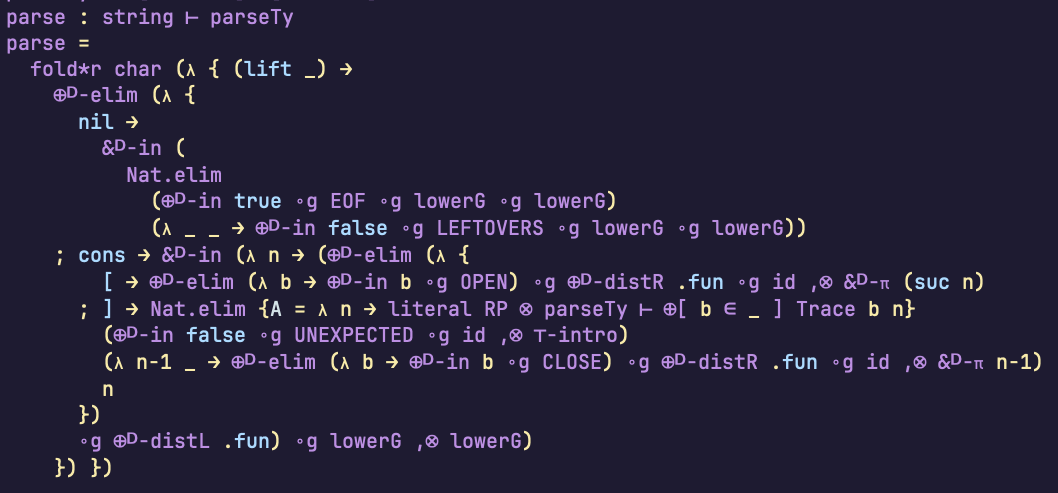
\includegraphics[width=\textwidth]{real_code.png}
  }
\end{frame}

\begin{frame}{Parsers Implemented in Agda}
\onslide<1->{
Dyck grammar (LL(0))
}

\onslide<2->{
Arithmetic expressions with a binary operation (LL(1))
}

\onslide<3->{
Regular expressions
\begin{itemize}
  \item Equivalences between NFAs, DFAs, and regexes
  \item Thompson's construction, powerset construction
\end{itemize}
}
\end{frame}


\section{Future Work}

\begin{frame}{Future Work}
  Parsing
  \begin{itemize}
    \item<+-> LL/LR parser generator
    \item<+-> Semantic actions
  \end{itemize}

  \onslide<+->{Implementation}
  \begin{itemize}
    \item<+-> Performance, ergonomics
  \end{itemize}

  \onslide<+->{Typechecking}
\end{frame}

\begin{frame}{Dependent Lambek Calculus}
\begin{center}
  \begin{tabular}{cc}
    \textbf{Grammars} & \textbf{Linear Types} \\
    \hline
    Grammar $A$ & Linear type $A$ \\
    \onslide<1->{ Parse of string $w$} & \onslide<1->{$w \vdash A$} \\
    \onslide<1->{ Parser } & \onslide<1->{$String \vdash A \oplus A_{\neg}$} \\
    \onslide<1->{ Parse transformer } & \onslide<1->{$\Delta \vdash A$} \\
  \end{tabular}
\end{center}

Implemented in Cubical Agda \agdalogo
\begin{itemize}
  \item {\small \url{https://github.com/maxsnew/grammars-and-semantic-actions}}
\end{itemize}

Preprint of this work
\begin{itemize}
  \item {\small \url{https://maxsnew.com/docs/lambek.pdf}}
\end{itemize}
\end{frame}

\end{document}
